\chapter{A hereditariedade e as características}\label{ch:g9:heredity-and-traits}

As fotografias de família são dados de \omterm{def:g1:living-or-not:living}{biologia}. O queixo da
avó no netinho, os cachos da mãe em nenhum dos dois filhos,
um irmão alto e o outro não --- a semelhança corre nas
famílias, e a diferença também. Este livro se apoia nesse
fato há anos (o potro da
\cref{rem:g4:animal-reproduction:mix}, os irmãos da
\cref{prop:g8:sexual-reproduction:shuffle}); o capítulo de
abertura deste ano finalmente a estuda: o que exatamente é
herdado, o que não é, e o que os padrões de semelhança
familiar nos deixam concluir.

\begin{omfigure}
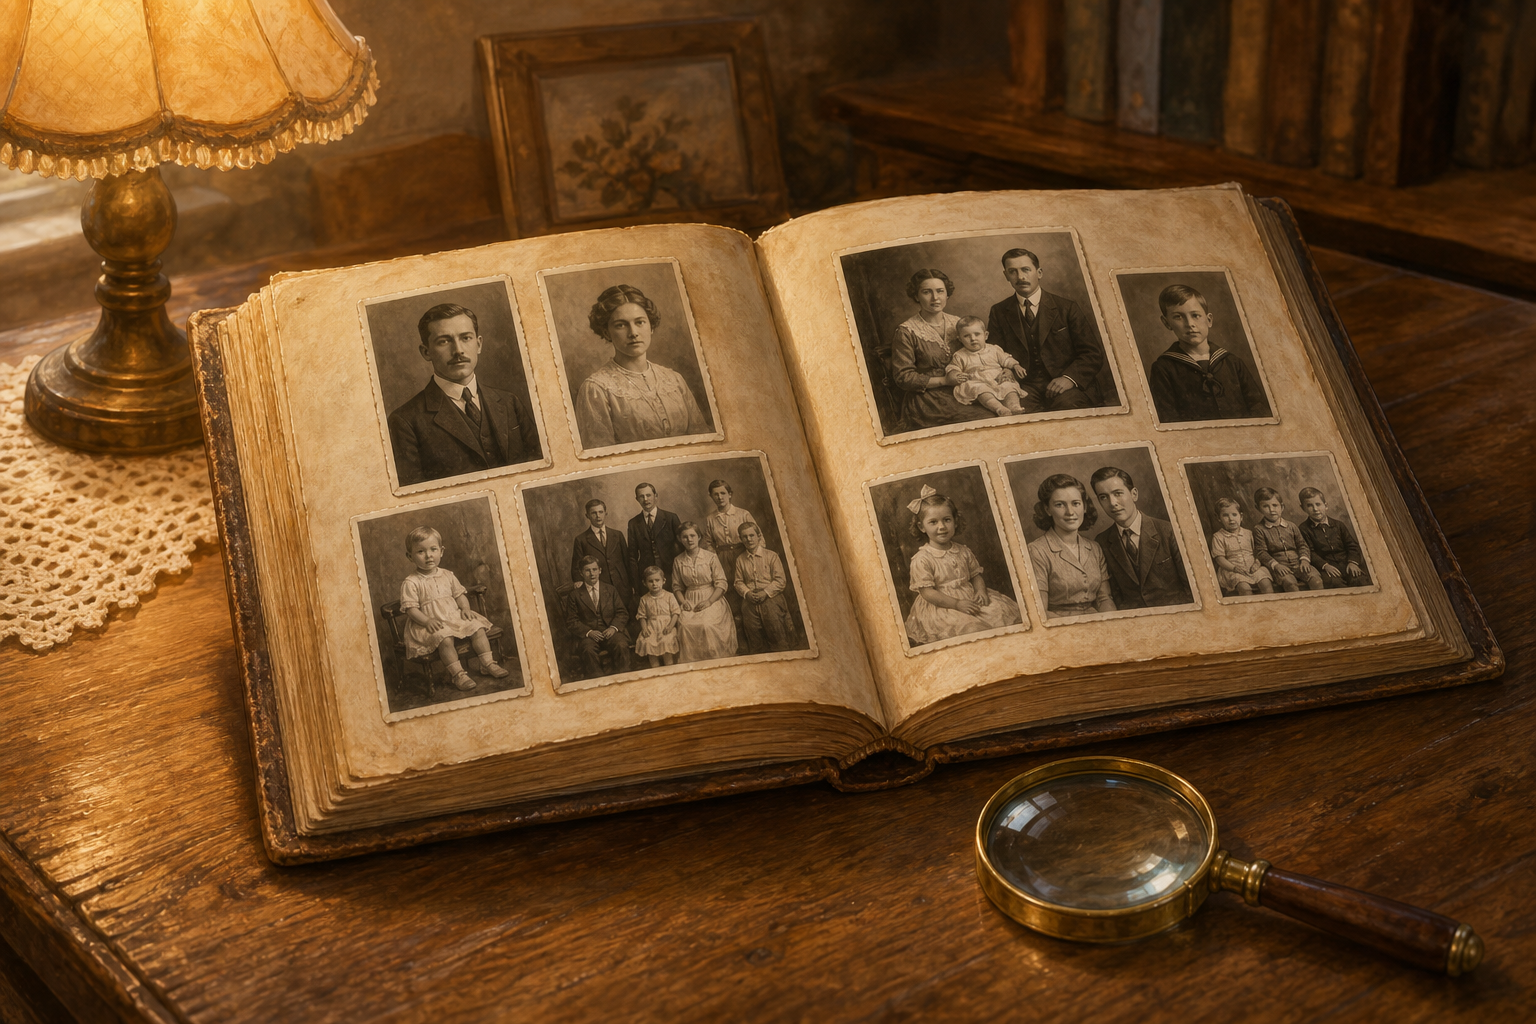
\includegraphics[width=0.62\linewidth]{images/book1/ai/g9-family-album.png}

{\small Dados de \omterm{def:g1:living-or-not:living}{biologia}, edição em sépia: a semelhança e a
diferença correndo pelas gerações.}
\end{omfigure}

\section{As características e de onde elas vêm}

\begin{definition}[As características]\label{def:g9:heredity-and-traits:traits}
Uma \emph{característica}\index{característica} é qualquer
traço descritível de um indivíduo: a cor dos \omterm{def:g1:the-five-senses:sense}{olhos}, o grupo
sanguíneo, o formato do lóbulo da orelha, a altura, uma voz
de cantar, uma cicatriz. O conjunto inteiro das
características de um indivíduo é construído por dois
trabalhos: o que foi \emph{herdado} e o que o \emph{\omterm{def:g6:exploring-our-environment:components}{ambiente}
e a vida} acrescentaram (o mundo da
\cref{def:g4:adapted-to-their-world:adaptation}, agindo
sobre um corpo só).
\end{definition}

\begin{definition}[A hereditariedade]\label{def:g9:heredity-and-traits:heredity}
A \emph{hereditariedade}\index{hereditariedade} é a
transmissão de \omterm{def:g9:heredity-and-traits:traits}{características} dos pais para os filhos pela
reprodução --- por meio de duas \omterm{def:g5:first-look-at-cells:cell}{células} isoladas, como
mostrou o \cref{ch:g8:sexual-reproduction}. As
\omterm{def:g9:heredity-and-traits:traits}{características} que passam por esse caminho são
\emph{hereditárias}\index{característica hereditária}: a cor
dos \omterm{def:g1:the-five-senses:sense}{olhos} e o grupo sanguíneo são; as cicatrizes e as
orelhas furadas não são, por mais tempo que sejam usadas. O
teste de triagem são os \omterm{def:g8:sexual-reproduction:gametes}{gametas}: o que duas \omterm{def:g5:first-look-at-cells:cell}{células} não
conseguem carregar, as famílias não conseguem transmitir.
\end{definition}

\begin{example}[Triando um álbum de família]\label{ex:g9:heredity-and-traits:album}
As fotografias do avô: o nariz marcante dele ---
hereditário, ei-lo de novo na tia e no primo; o bronzeado
curtido de lavrador --- adquirido, o neto que trabalha em
escritório não o tem; a altura dele --- em parte os dois,
pois o neto o ultrapassa na mesma armação, alimentado por
anos mais fartos (\cref{prop:g3:balanced-diet:jobs}); a
habilidade dele no violino --- não hereditária enquanto
habilidade (\cref{ex:g8:nervous-communication:juggler}: as
\omterm{def:g8:nervous-communication:synapse}{sinapses} são treinadas, e não transmitidas), embora a
família musical nos diga que algo mais sutil age no que é
passado adiante: talvez a aptidão, jamais a própria
instalação treinada.
\end{example}

\begin{proposition}[Herdado e adquirido]\label{prop:g9:heredity-and-traits:sorting}
Os dois trabalhos se separam em três testes:
\begin{enumerate}
  \item \emph{padrão familiar}: as \omterm{def:g9:heredity-and-traits:heredity}{características
        hereditárias} reaparecem pela árvore ao longo das
        linhas da reprodução; as adquiridas seguem as vidas
        (todos os marinheiros ficam curtidos, sejam quais
        forem os pais);
  \item \emph{presença desde o início}: o grupo sanguíneo
        fica fixado na \omterm{def:g5:flower-to-fruit:steps}{fecundação}; o bronzeado e a
        habilidade são construídos depois;
  \item \emph{transmissão}: os filhos de amputados têm os
        \omterm{def:g1:my-body:parts}{membros} deles; os filhos de fisiculturistas começam
        sem treino. As \omterm{def:g9:heredity-and-traits:traits}{características} adquiridas morrem
        com quem as adquiriu --- os \omterm{def:g8:sexual-reproduction:gametes}{gametas} não as carregam.
\end{enumerate}
A maioria das \omterm{def:g9:heredity-and-traits:traits}{características} visíveis --- a altura, a
compleição, até o temperamento --- é tecida pelos dois
trabalhos: uma faixa herdada e um preenchimento vivido.
\end{proposition}
\admitted

\section{Lendo os padrões de família}

\begin{example}[Características que pulam uma geração]\label{ex:g9:heredity-and-traits:skip}
Alguns padrões intrigam à primeira vista: dois pais de \omterm{def:g1:the-five-senses:sense}{olhos}
castanhos com um filho de \omterm{def:g1:the-five-senses:sense}{olhos} azuis; a \omterm{def:g9:heredity-and-traits:traits}{característica} da
avó ausente em todos os filhos e ainda assim de volta num
neto. Pular é comum, e isso carrega uma conclusão pesada: um
pai ou uma mãe pode \emph{transmitir o que não mostra}. As
instruções da \omterm{def:g9:heredity-and-traits:traits}{característica} viajaram escondidas por uma
geração --- então o que se herda não é a \omterm{def:g9:heredity-and-traits:traits}{característica} em
si, mas algo que a \emph{determina}, carregável sem ser
visto.
\end{example}

\begin{proposition}[O que os padrões nos obrigam a concluir]\label{prop:g9:heredity-and-traits:conclusions}
Três conclusões, cada uma obrigada por uma observação:
\begin{enumerate}
  \item já que as \omterm{def:g9:heredity-and-traits:traits}{características} adquiridas não passam, o
        que passa devem ser \emph{determinantes} ---
        instruções para construir \omterm{def:g9:heredity-and-traits:traits}{características}, e não as
        \omterm{def:g9:heredity-and-traits:traits}{características} em si;
  \item já que as \omterm{def:g9:heredity-and-traits:traits}{características} pulam gerações, os
        determinantes podem ser \emph{carregados sem
        aparecer}: cada indivíduo carrega mais do que exibe;
  \item já que cada filho recebe dos dois pais por dois
        \omterm{def:g8:sexual-reproduction:gametes}{gametas}
        (\cref{prop:g8:sexual-reproduction:core}), cada um
        deles contribui com uma \emph{seleção} dos
        determinantes que tem --- e as seleções diferem de
        filho para filho, senão os irmãos seriam iguais (o
        embaralhamento da
        \cref{prop:g8:sexual-reproduction:shuffle}, agora
        localizado: é um embaralhamento \emph{de
        determinantes}).
\end{enumerate}
\end{proposition}
\admitted

\begin{remark}[A pergunta que isso propõe]\label{rem:g9:heredity-and-traits:question}
O álbum de família nos encurralou numa pergunta maravilhosa.
Em algum lugar do quase-nada de um \omterm{def:g8:reproductive-systems:male}{espermatozoide}
(\cref{ex:g8:reproductive-systems:sperm} --- um \omterm{def:g6:cell-unit-of-life:parts}{núcleo}
compactado e uma cauda) viajam instruções para um nariz, um
grupo sanguíneo, uma cor de \omterm{def:g1:the-five-senses:sense}{olhos} --- carregáveis sem
aparecer, selecionáveis pela metade, legíveis pelo corpo que
cresce. \emph{Onde elas estão, e do que são feitas?} A
anatomia do \omterm{def:g8:reproductive-systems:male}{espermatozoide} já aponta a resposta: tudo o que
o pai manda cabe num \omterm{def:g6:cell-unit-of-life:parts}{núcleo} (a
\cref{rem:g5:first-look-at-cells:nucleus} prometeu que
aquele ponto importava). Os dois próximos capítulos o abrem.
\end{remark}

\begin{method}[Auditando uma característica]\label{met:g9:heredity-and-traits:audit}
Para qualquer \omterm{def:g9:heredity-and-traits:traits}{característica}, faça os três testes:
\begin{enumerate}
  \item mapeie-a na árvore genealógica: ela segue as linhas
        da reprodução, ou as vidas e os hábitos?
  \item date-a: fixada desde o início, ou construída pelo
        caminho?
  \item aplique o teste do \omterm{def:g8:sexual-reproduction:gametes}{gameta}: duas \omterm{def:g5:first-look-at-cells:cell}{células} poderiam
        carregá-la? (uma cicatriz não pode; um grupo
        sanguíneo pode);
  \item veredito: herdada, adquirida ou --- o mais comum ---
        uma faixa herdada, preenchida pela vida.
\end{enumerate}
\end{method}

\section{Exercícios}

\begin{exercise}[$\star$]\label{exo:g9:heredity-and-traits:1}
Defina \omterm{def:g9:heredity-and-traits:traits}{característica} e \omterm{def:g9:heredity-and-traits:heredity}{hereditariedade}, e dê o teste de
triagem numa frase só.
\end{exercise}

\begin{exercise}[$\star$]\label{exo:g9:heredity-and-traits:2}
Classifique: o grupo sanguíneo; uma orelha furada; as
sardas; o francês fluente; o formato do lóbulo da orelha.
\end{exercise}

\begin{exercise}[$\star$]\label{exo:g9:heredity-and-traits:3}
Enuncie os três testes da
\cref{prop:g9:heredity-and-traits:sorting}.
\end{exercise}

\begin{exercise}[$\star$]\label{exo:g9:heredity-and-traits:4}
Por que os filhos de fisiculturistas começam sem treino? O
que isso mostra?
\end{exercise}

\begin{exercise}[$\star$]\label{exo:g9:heredity-and-traits:5}
O que uma \omterm{def:g9:heredity-and-traits:traits}{característica} que pula uma geração prova que um
pai ou uma mãe consegue fazer?
\end{exercise}

\begin{exercise}[$\star$]\label{exo:g9:heredity-and-traits:6}
Por que o que é herdado tem de ser determinantes, e não
\omterm{def:g9:heredity-and-traits:traits}{características}? Uma frase.
\end{exercise}

\begin{exercise}[$\star\star$]\label{exo:g9:heredity-and-traits:7}
A altura veio maior no neto na mesma armação. Separe os dois
trabalhos que estão nessa frase.
\end{exercise}

\begin{exercise}[$\star\star$]\label{exo:g9:heredity-and-traits:8}
Explique por que os irmãos diferem, na linguagem dos
determinantes --- e por que os gêmeos idênticos
(\cref{exo:g8:from-egg-to-birth:10}) não diferem.
\end{exercise}

\begin{exercise}[$\star\star$]\label{exo:g9:heredity-and-traits:9}
Faça a \cref{met:g9:heredity-and-traits:audit} em: (a) os
cabelos brancos precoces que se repetem numa família; (b) o
fôlego de um jogador de futebol.
\end{exercise}

\begin{exercise}[$\star\star$]\label{exo:g9:heredity-and-traits:10}
O caso do violino: o que a família musical poderia estar
transmitindo, se nunca a habilidade treinada? Distinga com
cuidado.
\end{exercise}

\begin{exercise}[$\star\star$]\label{exo:g9:heredity-and-traits:11}
Dois pais de \omterm{def:g1:the-five-senses:sense}{olhos} castanhos, um filho de \omterm{def:g1:the-five-senses:sense}{olhos} azuis --- e
a vizinha desconfia da família. Defenda a família com a
lógica do \cref{ex:g9:heredity-and-traits:skip}.
\end{exercise}

\begin{exercise}[$\star\star\star$]\label{exo:g9:heredity-and-traits:12}
Só pela anatomia do \omterm{def:g8:reproductive-systems:male}{espermatozoide}
(\cref{ex:g8:reproductive-systems:sperm}), argumente onde os
determinantes do pai devem estar --- e que tamanho isso
implica para as instruções de um ser humano inteiro.
\end{exercise}

\section{Problema: A genealogista da aldeia}

\begin{problem}[{Problema de fim de semana --- três
gerações, um livro de características}]\label{pb:g9:heredity-and-traits:1}
Uma genealogista da aldeia anota as árvores genealógicas da
paróquia com \omterm{def:g9:heredity-and-traits:traits}{características}: o ``queixo da capela'' (um
queixo marcante que se repete há um século), a canhotice, a
tosse de \omterm{def:g7:how-animals-breathe:four}{pulmão} enfarinhado dos padeiros, os grupos
sanguíneos do registro de doações e os rostos curtidos dos
pastores.

\medskip\noindent\textbf{Parte I --- Triando o livro de
\omterm{def:g9:heredity-and-traits:traits}{características}.}
\begin{enumerate}
  \item Classifique as cinco \omterm{def:g9:heredity-and-traits:traits}{características} pela
        \cref{met:g9:heredity-and-traits:audit}, com o teste
        decisivo de cada uma.
  \item A tosse segue a padaria, e não a família: casar para
        dentro dela a traz, mudar-se para longe a perde. Que
        teste é esse, em ação?
  \item O queixo da capela pula a geração do meio em dois
        ramos. Tire a conclusão que isso obriga.
  \item Os grupos sanguíneos às vezes surpreendem o
        registro: um filho do grupo O de pais do grupo A e
        do grupo B. O que cada um dos pais deve ter
        carregado?
\end{enumerate}

\medskip\noindent\textbf{Parte II --- A leitura pelos
determinantes.}
\begin{enumerate}[resume]
  \item Reescreva o século do queixo na linguagem dos
        determinantes: o que de fato viajou por quatro
        gerações, e em que veículos
        (\cref{def:g9:heredity-and-traits:heredity})?
  \item Por que os primos que carregam o queixo diferem em
        todo o resto? Localize o embaralhamento.
  \item A genealogista não encontra nenhum caso --- num
        século --- de uma cicatriz, de um ofício ou de uma
        língua passando para um recém-nascido. Enuncie a
        generalização e a razão dela no nível do mecanismo.
  \item Os gêmeos de uma família combinam no queixo e em
        tudo o mais. O que o livro conclui sobre o começo
        deles (\cref{rem:g5:human-reproduction:twins})?
\end{enumerate}

\medskip\noindent\textbf{Parte III --- A palestra.}
\begin{enumerate}[resume]
  \item A genealogista dá uma palestra: ``a paróquia
        transmite duas heranças --- uma pelos \omterm{def:g8:sexual-reproduction:gametes}{gametas}, outra
        pelo convívio''. Distribua as cinco \omterm{def:g9:heredity-and-traits:traits}{características}
        do livro pelos dois canais.
  \item ``Cada um de nós exibe menos do que carrega.''
        Defenda essa frase a partir do livro, duas vezes.
  \item Um ouvinte pergunta o que são fisicamente as
        instruções do canal dos \omterm{def:g8:sexual-reproduction:gametes}{gametas}. Dê a resposta
        honesta da \cref{rem:g9:heredity-and-traits:question}
        --- localização conhecida, conteúdo no próximo
        capítulo.
  \item Encerre a palestra com o veredito de uma linha da
        auditoria sobre o caso mais comum: a maioria das
        \omterm{def:g9:heredity-and-traits:traits}{características} é \emph{o quê}, vivido \emph{como}?
\end{enumerate}
\end{problem}
